\documentclass{beamer}
%\usetheme{Berkeley}
%\usetheme{Boadilla}
%\usetheme{Madrid}
%\usetheme{Montpellier}
\usetheme{Warsaw}
%\usetheme{Copenhagen}
%\usetheme{Goettingen}
%\usetheme{Hannover}
%\usetheme{PaloAlto}
%\usetheme{AnnArbor}
%\usetheme{Bergen}

%\usepackage{beamerthemesplit}


\usepackage{amscd,amsxtra,amsthm}
%\usepackage[all]{xy}
%\usepackage{etex}
%\usepackage{pictex}
\usepackage{graphicx}
\usepackage{mathtools}

\theoremstyle{conjecture1}
%\newtheorem{conjecture}[theorem]{Conjecture}
\newtheorem{conjecture1}[theorem]{Conjecture 1}
\theoremstyle{conjecture2}
%\newtheorem{conjecture}[theorem]{Conjecture}
\newtheorem{conjecture2}[theorem]{Conjecture 2}

\def\G{\widetilde{G}}
\def\B{\widetilde{B}}
\def\T{\widetilde{T}}
\def\b{\widetilde{b_* }}
\def\M{\overline{M}}
\def\C{\mathbb{C}}
\def\Q{\mathbb{Q}}
\def\Z{\mathbb{Z}}
\def\F{\mathbb{F}}
\def\I{\mathbb{I}}
\def\Q{\mathbb{Q}}
\def\N{\mathbb{N}}
\def\R{\mathbb{R}}
\def\s{\mbox{\bf s}}
\def\pr{\mbox{\bf p}}
\def\i{\mbox{\bf i}}
\def\k{\mbox{\bf k}}
\def\h{\mbox{\bf h}}
\def\e{\epsilon}
\def\vp{\varpi }
\def\O{\mathcal{O}}
\def\v{\upsilon }
\def\p{\wp }
\def\z{\zeta _\upsilon}
\def\d{\cdot}
\def\c{\bullet}
\def\a{\ast}








\title{Chv\'atal's Theorem for Tree-Complete Ramsey Numbers}
\author[Mark Budden \\ \quad \\ Western Carolina University]{Mark Budden}
\date{August 28, 2021 \\ Sample Presentation for Math 479}

\begin{document}

\frame{\titlepage}







\section{Definitions and Examples}



\frame{
\begin{itemize}
	\item<1-> Recall that a {\bf tree} can be defined by one of several equivalent definitions.  In particular,
		\begin{itemize}
			\item<2-> A tree is a connected graph that does not contain any cycles.
			%\item<3-> A tree is a graph that is minimally connected (ie., it is connected, but the removal of any edge disconnects the graph).
			%\item<4-> A tree is a graph in which there exists a unique path between any distinct pair of vertices.
			\item<3-> A tree is a graph that can be constructed edge-by-edge, with each new edge including exactly one vertex from the previous graph (ie., the addition of each new edge requires the addition of one new vertex).
		\end{itemize}
		\hspace{.6in}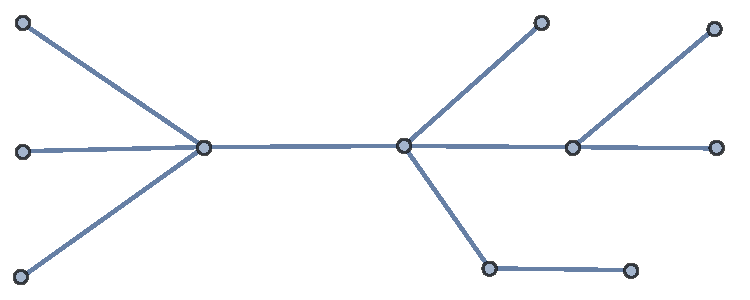
\includegraphics[scale=.5]{tree.pdf}
	\item<4-> From this second definition, it follows that every tree contains at least one {\bf leaf} (a vertex of degree one).	
\end{itemize}
}




\frame{
\begin{itemize}
	\item The {\bf complete graph} $K_n$ is a graph of order $n$ in which every pair of distinct vertices are adjacent.
\end{itemize}	

	\hspace{.5in}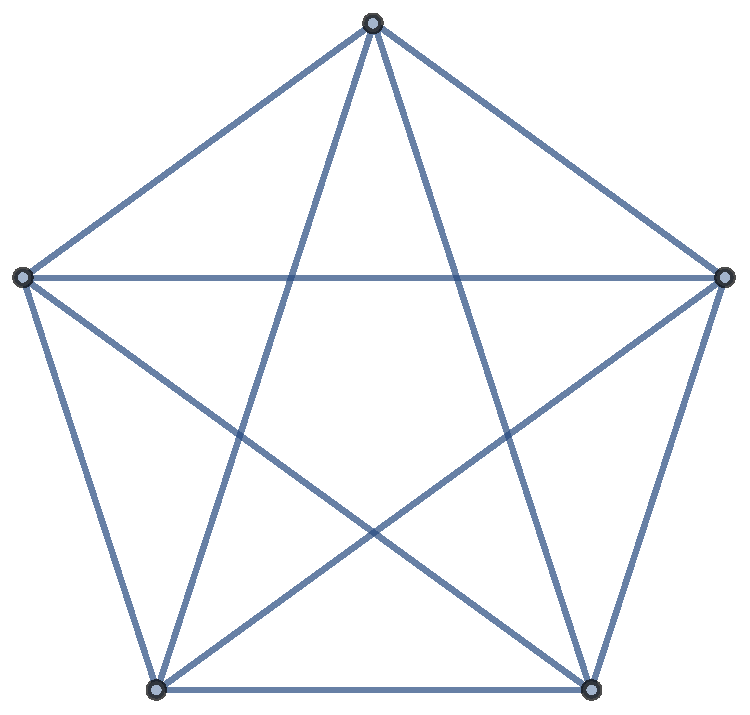
\includegraphics[scale=.3]{K5.pdf}\qquad  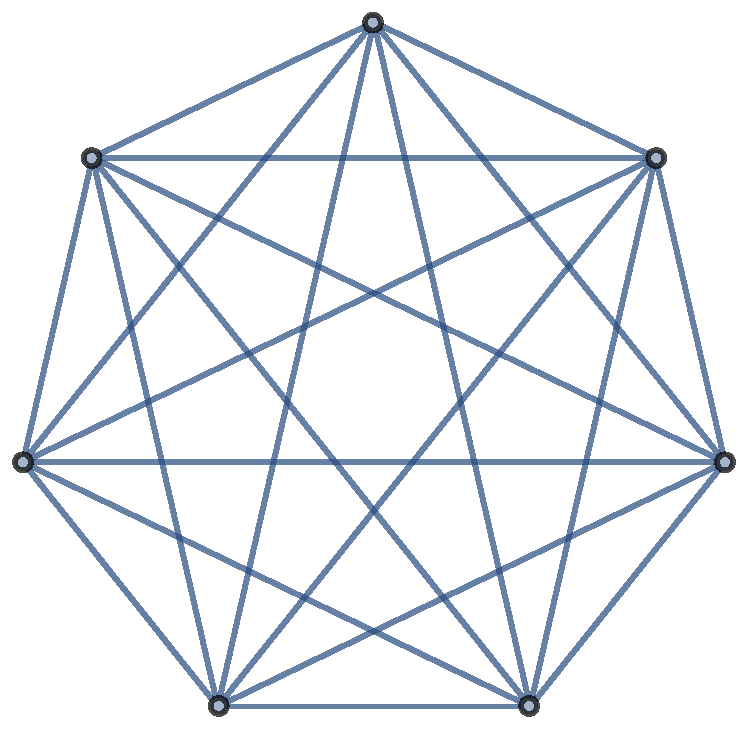
\includegraphics[scale=.3]{K7.pdf}
	
	\hspace{1.1in} $K_5$ \hspace{1.55in} $K_7$
}


\frame{
	\begin{itemize}
		\item<1-> The {\bf chromatic number} $\chi (G)$ of a graph $G$ is the minimum number of colors needed to color the vertices of $G$ so that no two adjacent vertices receive the same color.
		\item<2-> If $T$ is any tree containing at least one edge, then $\chi (T)= 2$.
		\item<3-> For all $n\in \N$, $\chi (K_n)=n$.
	\end{itemize}
}



\frame{
\begin{itemize}
	\item<1-> For any graphs $G_1$ and $G_2$, the {\bf Ramsey number} $R(G_1, G_2)$ is the least natural number $p$ such that every red/blue coloring of the edges of $K_p$ contains a red subgraph isomorphic to $G_1$ or a blue subgraph isomorphic to $G_2$.
	\item<2->  The existence of Ramsey numbers follows from Frank Ramsey's foundational work [4].
\end{itemize}
}



\frame{
\begin{itemize}
	\item<1-> Properties of $R(G_1, G_2)$:
	\begin{enumerate}
		\item<2-> $R(K_1, G_2)$\uncover<3->{ $=1$, for all graphs $G_2$.}
		\item<4-> $R(K_2, G_2)$\uncover<5->{ $=n$, for all graphs $G_2$ of order $n$.}
		\item<6-> $R(G_1, G_2)=R(G_2, G_1)$, for all graphs $G_1$ and $G_2$.
	\end{enumerate} 
\end{itemize}
}






\section{The Work of Chv\'atal and Harary}


\frame{
In 1972, Chv\'atal and Harary [2] proved the following theorem.
\begin{theorem}[Chv\'atal and Harary] For all graphs $G_1$ and $G_2$, $$R(G_1, G_2)\ge (c(G_1)-1)(\chi (G_2)-1)+1,$$ where $c(G_1)$ is the order of the largest connected component in $G_1$.
\end{theorem}
\begin{itemize}
	\item<2-> From this result, it follows that if $T_m$ is any tree of order $m$, then $$R(T_m, K_n )\ge (m-1)(n-1)+1.$$
\end{itemize}
}




\frame{
\begin{itemize}
	\item<1-> Observe that $T_1=K_1$ and $T_2=K_2$.
	\item<2-> We can confirm that the lower bounds proved by Chv\'atal and Harary are exact in the following cases:\begin{align} R(T_1,K_n)\ge (1-1)(n-1)+1=1, \notag \\ R(T_2, K_n)\ge (2-1)(n-1)+1=n. \notag 
\end{align}
	\item<3-> In fact, in 1977, Chv\'atal [1] proved that this is always the case.
\end{itemize}
}



\frame{
\begin{theorem}[Chv\'atal] For every tree $T_m$ of order $m$, $$R(T_m, K_n)=(m-1)(n-1)+1.$$
\end{theorem}
}





%\section{The Proof of Chv\'atal's Theorem}

\frame{\frametitle{The Proof of Chv\'atal's Theorem}
\begin{itemize}
	\item<1-> It remains to be shown that $$R(T_m, K_n)\le (m-1)(n-1)+1,$$ for all trees $T_m$ of order $m$.
	\item<2-> We proceed by (strong) induction on $m+n$.
	\item<3-> The Ramsey numbers $$R(T_1, K_n)=1=R(T_m, K_1)$$ are the base cases.
	\item<4-> Inductive hypothesis: suppose that $$R(T_{m'}, K_{n'})\le (m'-1)(n'-1)+1$$ for all $m'+n'<m+n$.
\end{itemize}
}

\frame{\frametitle{The Proof of Chv\'atal's Theorem}
\begin{itemize}
	\item<1-> Consider a red/blue coloring of the edges in $K_{(m-1)(n-1)+1}$.
	\item<2-> Let $T'$ be the tree formed by removing a single leaf from $T_m$ and denote by $x$ the vertex in $T'$ that was adjacent to the removed leaf.
	\item<3-> By the inductive hypothesis, $$R(T', K_n)\le (m-2)(n-1)+1<(m-1)(n-1)+1.$$
	\item<4-> It follows that there exists a red $T'$ or a blue $K_n$.  Suppose the former case.
\end{itemize}
}

\frame{\frametitle{The Proof of Chv\'atal's Theorem}
\begin{itemize}
	\item<1-> So, our coloring contains a red $T'$.  Other than the $T'$, there are $$(m-1)(n-1)+1-(m-1)=(m-1)(n-2)+1$$ other vertices.
	\item<2-> Applying the inductive hypothesis again, we find that $$R(T_m, K_{n-1})\le (m-1)(n-2)+1.$$
	\item<3-> Hence the two coloring of the remaining vertices contains either a red $T_m$ or a blue $K_{n-1}$.  Assume the latter case.
\end{itemize}
}

\frame{\frametitle{The Proof of Chv\'atal's Theorem}
\begin{itemize}
	\item<1-> Thus, the original red/blue coloring of $K_{(m-1)(n-1)+1}$ contains a red $T'$ and a blue $K_{n-1}$ that are disjoint.
	
	 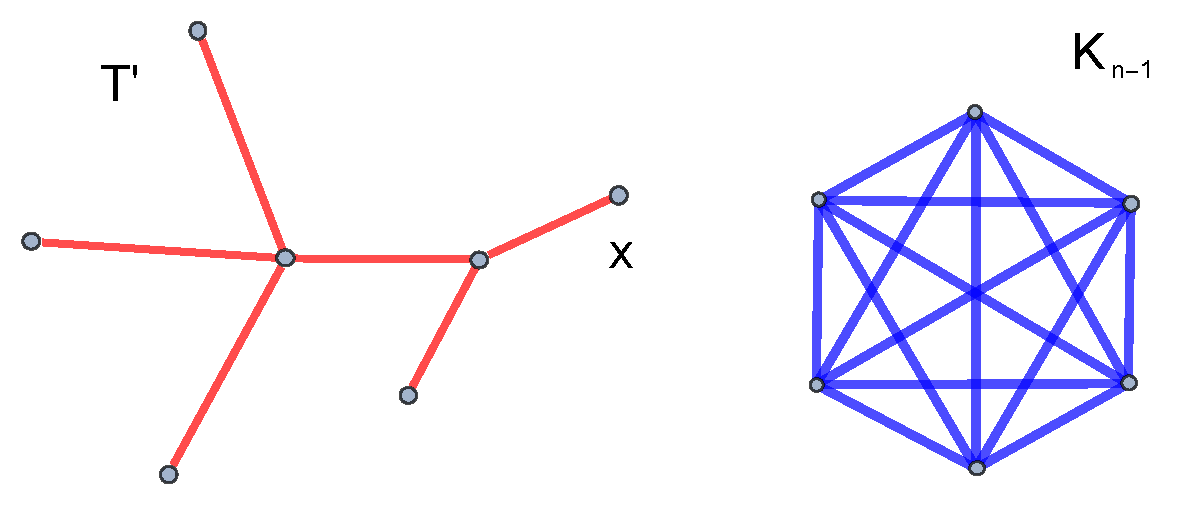
\includegraphics[scale=.5]{treecomplete1.pdf}
	 \item<2-> Consider the edges connecting $x$ to the vertices in the blue $K_{n-1}$.
\end{itemize}
}

\frame{\frametitle{The Proof of Chv\'atal's Theorem}
 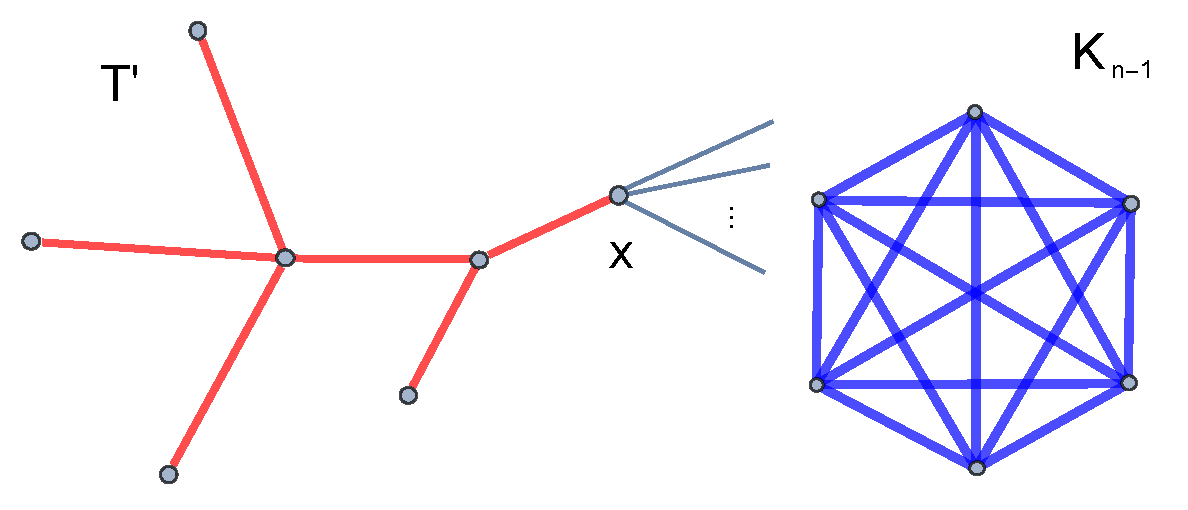
\includegraphics[scale=.5]{treecomplete2.pdf}
\begin{itemize}
	\item<2-> If any such edge is red, then we obtain a red subgraph isomorphic to $T_m$.
	\item<3-> Otherwise, all such edges are blue, and a blue $K_n$ is formed.
\end{itemize}
}

\frame{\frametitle{The Proof of Chv\'atal's Theorem}
\begin{itemize}
	\item<1-> We have proved that every red/blue coloring of $K_{(m-1)(n-1)+1}$ contains a red $T_m$ or a blue $K_n$.
	\item<2-> Hence, $$R(T_m, K_n)\le (m-1)(n-1)+1,$$ completing the proof of the theorem. \hspace{1.4in}$\square$
\end{itemize}
}

\section{Conclusion}







\frame{
Concluding Remarks:
\begin{enumerate}
	\item<1-> A similar proof using induction can be used to show that $$R(T_m, K_{1,n})\le m+n-1,$$ where $K_{1,n}$ is a star (a tree with $n$ leaves and one vertex of order $n$).
	\item<2-> When a connected graph $G$ of order $m$ satisfies $$R(G, K_n)\le (m-1)(n-1)+1,$$ it is called {\it $n$-good}.  Ongoing research focuses on classifying all $n$-good graphs.
	%\item<3-> Results similar to those of Chv\'atal and Harary exist for hypergraphs, but few explicit evaluations of the corresponding Ramsey numbers are known.
\end{enumerate}
}





%\frame{Tightness, Chromatic numbers, ... , spanning minimally connected hypergraph, rainbow connected, connectedness in general, $n$-good}


\frame{
\frametitle{References}
\begin{enumerate}{\scriptsize
%\item Budden, Hiller, and Penland, {\it Minimally Connected Hypergraphs,} in preparation.
%\item Budden and Penland, {\it Trees and $n$-Good Hypergraphs,} under review.
%\item Burr, {\it Generalized Ramsey Theory for Graphs - A Survey,} Graphs and Combinatorics, Springer-Verlag, Berlin (1974), 52-75.
%\item Burr, {\it Ramsey Numbers Involving Graphs with Long Suspended Paths,} J. London Math. Soc. (2) {\bf 24} (1981), 405-413.
%\item Burr and Erd\H{o}s,  {\it Generalizations of a Ramsey-Theoretic Result of Chv\'atal,} J. Graph Theory {\bf 7} (1983), 39-51.
\item[{[1]}] Chv\'atal, {\it Tree-complete Graph Ramsey Numbers,} J. Graph Theory {\bf 1} (1977), 93.
\item[{[2]}] Chv\'atal and Harary, {\it Generalized Ramsey Theory for Graphs III, Small Off-diagonal Numbers,} Pacific J. Math. {\bf 41} (1972), 335-345.  
\item[{[3]}] Radziszowski, {\it Small Ramsey Numbers,} Elec. Journ. of Combin., Dynamic Survey {\bf 1}, last updated 2017.
\item[{[4]}] Ramsey, {\it On a Problem of Formal Logic,} Proc. London Math. Soc. {\bf 30} (1930), 264-286.

}\end{enumerate}
}


%%%%%%%%%%%%%%%%%%%%%%%%%%%%%%%%%%%%%%%%%%%%%%
%%%%%%%%%% End completed part of talk %%%%%%%%%%%%%%%%%%%%%%
%%%%%%%%%%%%%%%%%%%%%%%%%%%%%%%%%%%%%%%%%%%%%%


%%%%%%%%%%%%%%%%%%%%%%%%%%%%%%%%%%%%%%%%%%%%%%%%%%%%%%%%%%%%%%%%%%%%%%%%%%%%%%%%%%


%\section{Project Description}
%\subsection{Overview of the Beamer Class}
%\frame{
%  \frametitle{Features of the Beamer Class}

%  \begin{itemize}
%  \item<1-> Normal LaTeX class.
%  \item<2-> Easy overlays.
%  \item<3-> No external programs needed.
%  \end{itemize}
%}


\end{document}
